%2345678901234567890123456789012345678901234567890123456789012345678901
% chapter radamscharobs (fold)
\chapter[RADAMS: Characterising radio astronomical observations]
[RADAMS: Characterising radio observations]
{RADAMS: Characterising radio astronomical observations} 
\label{cha:radamscharobs}
	
	\invisiblenote{
		The most important data model to implement is the CharDM.
		Characterisation allows systems querying a VO registry to
		find which datasets contain some data of interest (because
		of the region of the sky, the spectral band, sensibility,
		et cetera), and later on evaluate if the query results are
		indeed of interest.
		
		 In this chapter we will develop the Characterisation data
		model for radio astronomical observations,
		
		 After this initial overview of the classes that conform
		the RADAMS, we will detail the attributes corresponding to
		each of the classes of the model.
	}
	
	In the previous chapter we analysed how an astronomical archive
	could be built using the basis of the ObsDM, if the missing
	data models suggested by the ObsDM document were to be
	implemented. We also illustrated how VO compatibility could be
	added to archives built on such a basis much more easily.
	
	After that, we showed the high level overview of the RADAMS,
	which was at first glance almost indistinguishable from the
	ObsDM, something which is indeed a feature of the RADAMS.
	Finally, we provided a first overview of the definition of
	each particular class and sub-models, and the way they mesh
	together.
	
	Once we have introduced the RADAMS,  we will start studying it
	in detail in this and the following chapters.  In particular,
	this chapter will be devoted to how the RADAMS stores the
	Observation and ObsData information, and how the 
	CharDM data model is filled for the different observation
	modes in radio telescopes.
	
	In addition, in those chapters devoted to the
	detailed exploration of the RADAMS, we will select appropriate
	FITS Keywords  and UCDs for FITS and VOTable serialisations of
	observational data.  FITS Keywords will be selected first from
	the official FITS mandatory headers~\cite{Hanisch:1999fk}.  If
	no mandatory   keyword exists,   they will be chosen  from the
	Multi-Beam FITS Raw Data Format~\cite{MudPolHat0512Multi-Beam},
	and lastly from the NRAO GBT FITS data
	format~\cite{PreCla0412Device}\footnote{Sometimes those
	keywords cannot appear in the main header of a FITS file, but
	instead in a FITS extension table, but that will not be
	specified.}. Where \texttt{assign} appears, it means
	that a suitable FITS keyword has yet to be
	selected for that particular database attribute.
	
	UCDs will be selected from the UCD1+
	vocabulary~\cite{2005ucv..rept.....P}, using the recommended
	juxtaposition technique in order to clarify the meaning of any
	given term. In some cases, there are no existing UCD atoms, and
	no UCD atom combination, properly describing the attribute. In
	those cases, we will propose corresponding UCD unique atoms,
	for stand-alone or combined use.
	
	We also want to acknowledge the initial effort by Lamb
	and Power in creating a draft for an IVOA
	Note~\cite{LamPow0310IVOA} in which radio astronomical data were
	initially modelled. Many of the controlled vocabularies
	proposed in this and the following chapters have used that
	document as a source.
	
	\invisiblenote{
		char•ac•ter•ize |ˈkariktəˌrīz| 
		verb [ trans. ] 
		1 describe the distinctive nature or features of : the historian characterized the period as the 
		decade of revolution. 
		2 (often be characterized) (of a feature or quality) be typical or characteristic of : 
		the disease is characterized by weakening of the immune system. 

		ob•serve |əbˈzərv| 
		verb [ trans. ] 
		1 notice or perceive (something) and register it as being significant : [with clause ] 
		young people observe that decisions are made by others. 
		• watch (someone or something) carefully and attentively : Rob stood in the hallway, 
		where he could observe the happenings on the street. 
		• take note of or detect (something) in the course of a scientific study : the behavior 
		observed in groups of chimpanzees. 

		ob•ser•va•tion |ˌäbzərˈvā SH ən| 
		noun 
		1 the action or process of observing something or someone carefully or in order to 
		gain information : she was brought into the hospital for observation | detailed observations 
		were carried out on the students' behavior. 
		• the ability to notice things, especially significant details : his powers of observation. 
		• the taking of the altitude of the sun or another celestial body for navigational 
		purposes. 
	}
	
	\section{ObsData and Characterisation} %(fold)
	\label{subObsDataCharacterisation}
		
		Following the IRAM MultiBeam FITS definition
		document~\cite{MudPolHat0512Multi-Beam}, based on the ALMA
		Software Glossary~\cite{Schwarz:2003zr}, we can define
		several degrees of observational data in radio astronomy:
		
		\begin{description}
			\item[Dump] This is the smallest interval of time for
			which a set of correlated data can be accumulated and
			output from the backend stage.
			
			 \item[Integration] Set of dumps, all identical in
			configuration, which are accumulated and form the basic
			recorded unit.
			
			 \item[Sub-scan] Set of integrations performed while
			the antennas complete an elemental pattern across the
			source: e.g., an azimuth displacement on a pointing 
			source, a focus displacement within a focus calibration,
			et cetera.
			
			 \item[Scan] Set of sub-scans with a common goal, such
			as a pointing scan, a focus scan or an atmospheric
			amplitude calibration scan, among others.
		\end{description}
			
		Hence, the minimum useful unit to be recorded in the
		archive is the sub-scan, which can be appropriately
		described, but the minimum scientifically significant unit
		is the scan, so depending on the kind of granularity
		desired one could base the archive upon one or the other.
		Higher order units ---such as multiple scans on the same
		source, for enhancing the signal-to-noise ration, or
		scans to different sources belonging to the same observing 
		program--- should be derived from Project metadata.
		
		 To link together these scans with the rest of the data model
		we will use the ObsData class
		(which could also be referred to as \classname{RawData}) as the root
		class for the RADAMS. From ObsData instances, we will form
		a tree of data that will describe a particular scan, both
		by its properties in the Spatial, Temporal, Spectral, and
		Observable axes, and its respective Accuracy.
		
		 We show a high level overview of the ObsData class and its
		relationships with AxisFrame, Coverage, Resolution, and
		Accuracy classes in figure~\ref{figObsData}. Compare it 
		with figures~\ref{fig:fig_CharDMPerAxisProperties} and
		\ref{fig:fig_CharDMAccuracy}.
		
		
		\begin{figure}[tbp]
		\begin{center}
		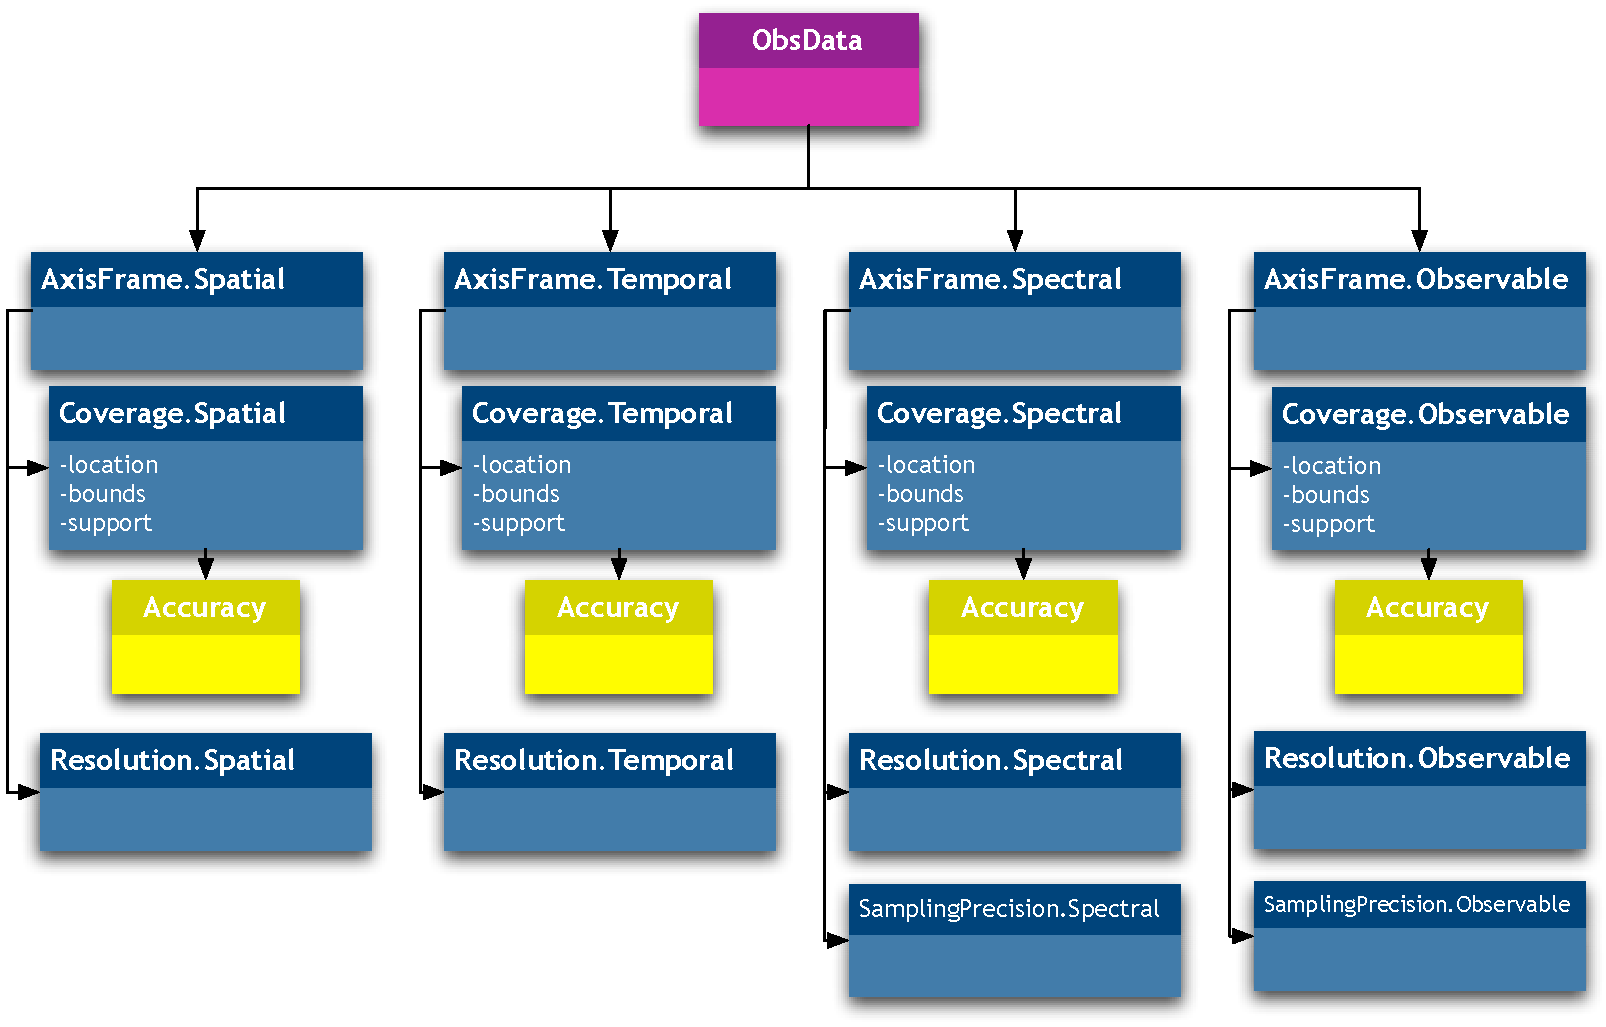
\includegraphics[width=\columnwidth]{fig/ObsData-DM}
		\end{center}
		\caption[ObsData class data model]{
			ObsData class data model; the different axes for the
			Characterisation part of the data model are shown.
		}
		\label{figObsData}
		\end{figure}
		
		\begin{description}
			\item[ObsData] Instances of this class (also to be
			referred as RawData) will contain the final data. As
			discussed previously, we will keep either whole scans
			to determine the scientific data, or processed data
			(such as spectra).
		
			 \item[AxisFrame] Instances of this class will contain
			metadata that describe properties of the axis,
			such as units, calibration state, et cetera.
		
			 \item[Coverage] We will describe the position of the
			archived data in the parameter space: where and when was
			the telescope pointed, and what wavelength range was
			observed. Several subclasses exist:
		
			\begin{description}
				\item[Location] This subclass of each Coverage
				axis
				describes the characteristic value for each of
				them.
				For instance, in the spatial axis
				Coverage.Spatial.Location would be set to
				the central point of the observed field, and for
				the temporal axis
				Coverage.Temporal.Location would hold 
				either the middle or the start
				time of the scan.
				
				\item[Bounds] Maximum and minimum values
				of the axis; for instance, Coverage.Spectral.Bounds
				would give us the maximum and minimum frequencies
				of the spectrum, and Coverage.Tem\-po\-ral.Bounds
				would give us the starting and ending time of the
				observation.
				
				\item[Support] Set of parameters in that
				axis where we have valid observational data. For
				instance, in the temporal axis
				Coverage.Tem\-po\-ral.Sup\-port could be
				a set of intervals when data were gathered,
				excluding the pauses for reissuing scans.
				
				\item[Sensitivity] Sensitivity is an
				additional refinement to Support, where for the
				sections of the axis with Support for the observation
				a response function of the instrument in
				the given axis is provided.
				This is especially useful for cases with a large
				number of small interruptions in the data, there is
				need for data resampling, filter
				profiles have to be accounted for, and so on.
			\end{description}
			
			We have to remember that these subclasses form a
			hierarchy by which Location is mandatory, and all
			further refinements optional, but for a refinement
			to appear all levels above it must appear to: for
			instance, we can provide just Location, but if Support
			appears, Bounds needs to appear as well.
		
			\item[Resolution] Instances of this class are used to
			describe resolution in each axis. For instance,
			Coverage.Spatial.Resolution would be defined in 
			single-dish observations by the Half-Power Beam
			Width (HPBW).
			
			 \item[SamplingPrecision] For a sampled axis ---such as
			the Spectral axis, in the case of spectroscopic
			data---, an instance of this class will hold sampling
			precision, described as a pixel scale.
			
			 \item[Accuracy] All of the aforementioned classes
			should have an accompanying class in order to describe
			errors and data quality for each axis. In the case of
			archives without data mining capabilities, we only have
			to provide Accuracy instances related to the Coverage
			classes.
			
		\end{description}
		
		\invisiblenote
		{\textbf{Refine this paragraph with better description of
		errors and their handling.} It has to be noted that, for
		some observational sets, there is no meaningful definition
		of an error. Instead, one can define statistical error
		estimations valid for a certain period, and apply those
		definitions for observations being performed during said
		period. That would be the case, for instance, of errors in
		pointing or focus, where one cannot specify the error for a
		single observation, but pointing or focus error averages.}
		
		\subsection{AxisFrame.Spatial and Coverage.Spatial} % (fold)
		\label{ssubSpatialAxis}
			
			In this subsection, we describe the classes that
			configure the description of the spatial axis
			(AxisFrame.Spatial), and the characterisation of the
			coverage in such axis (Coverage.Spatial).
			Figure~\ref{figAxisFrameSpatial} shows the classes and
			their relationships.
			
			\begin{figure}[tbp]
			\begin{center}
			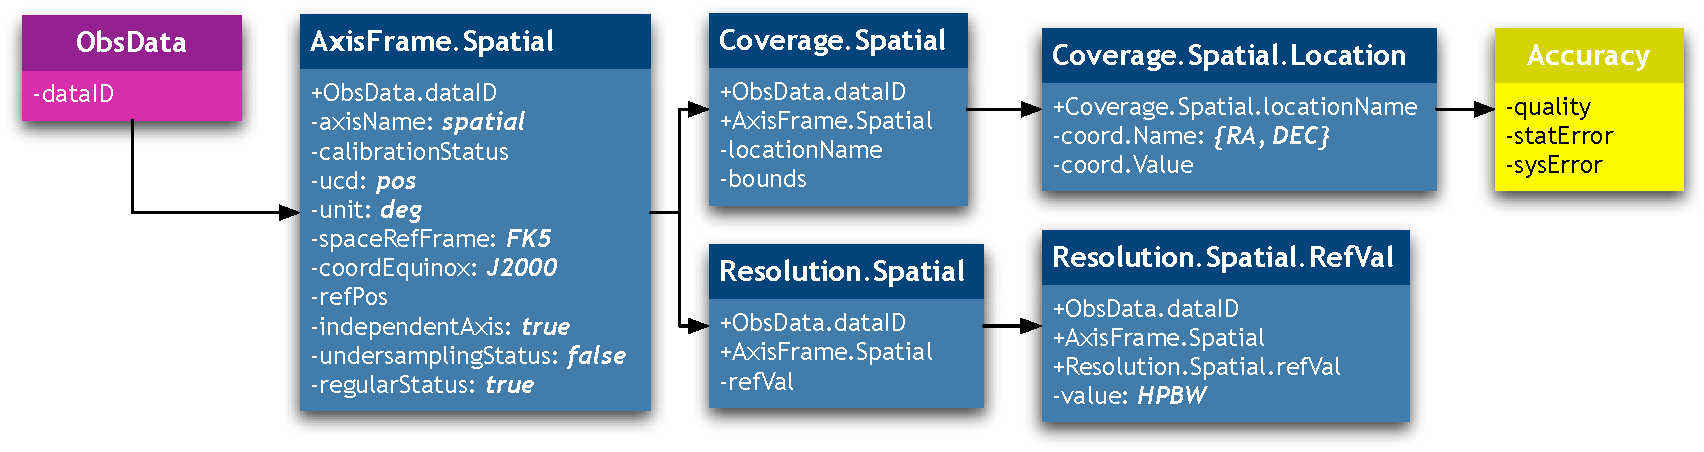
\includegraphics[width=\columnwidth]
			{fig/AxisFrame-Spatial-DM}
			\end{center}
			\caption[Spatial axis frame metadata]
			{
				Spatial axis frame and coverage metadata.
				\todoinlinesuspended{Redo figure with Bounds, Support,
				Sensitivity.}
			}
			\label{figAxisFrameSpatial}
			\end{figure}

			\begin{description}
				\item[AxisFrame.Spatial] This instance describes
				the properties of the Spatial axis, such as
				calibration status, units (normally, degrees),
				reference frame, epoch, spatial sampling type and
				sampling status, et cetera.
				
				 For the DSS-63 antenna, the spatial axis is never
				sampled (because we are not storing maps at this
				stage), and each scan only needs two pairs of
				coordinates (plus pointing accuracy) to describe
				the antenna-pointing pattern.
				
				\invisiblenote{Redo discussion, taking into account
				mappings, and the enhancements for interferometry.}
				
				 As the coordinate space is in this case
				bi-dimensional, and properties for one of the
				coordinates do not have to be equal for the other,
				we should either choose between a vector approach,
				using two dimensional arrays of coordinates, or
				splitting the Spatial classes in different
				subclasses. We choose the first approach, and thus
				all AxisFrame.Spatial attributes will have a
				space-separated array of values (just two values
				separated with an space, for a bi-dimensional
				coordinate space).
				
				 If the archive were to be exploited in the third
				dimension, an additional distance and/or redshift
				coordinate should be entered. As we have seen,
				extension in the spatial axis is straightforward. A
				second option would add an additional axis to the
				Characterisation data model.
				
				 \item[Coverage.Spatial.Location] For the DSS-63
				antenna, the stored values for this class
				correspond to the antenna pointing coordinates.
				If a Target is linked, Spatial.Location information
				sould be the same, unless the target is not directly
				associated, but found by
				cross-correlation with the Targets database.
				
				 \item[Coverage.Spatial.Bounds] Bounds for spatial
				data would be the maximum and minimum for spatial
				coordinates (normally, right ascension and
				declination) when observing the source. For single
				point spectroscopic data, this class is not needed,
				as the antenna does not describe any path across
				the source.
				
				 \item[Coverage.Spatial.Support] Typically, the
				stored values for this class should be equal to
				those of Coverage.Spatial.Bounds, except when
				invalid data within Coverage.Spatial.Bounds might
				exist, or in order to describe an elaborate
				scanning path on the source. This class would
				describe such a path.
				
				 \item[Coverage.Spatial.Sensitivity] In the case of
				the DSS-63 antenna, Spatial.Sen\-si\-tivity would
				be defined as the beam pattern of the antenna,
				in principle in 1D taking symmetries into account,
				but 2D could be considered, as it would be the
				case for a synthesised beam in interferometry.
				Another possibility is the combination of beam
				pattern with receiver efficiency at different
				elevations.
			\end{description}
			
			\invisiblenote
			{\textbf{Rewrite taking into account OTFs, and mappings.
			We already have tables for Spatial.Bounds, .Support
			and even .Sensitivity.}
			Bear in mind that Coverage.Spatial.Support for radio
			astronomical measurements is either a point, for
			spectroscopic calibrations, or a set of line paths for
			bolometric and/or continuum mappings. Spatial support
			will be defined as the set of line paths, and can be
			described by an array of start/end value pairs for 2D sky
			coordinates\footnote{In fact, that is exactly the way 
			paths across the sky for OTF observations are stored
			by the IRAM~30m New Control System.}.
			
			 For spectroscopic data, this class is redundant, as
			mentioned above.}
			
			\begin{table}
			\begin{minipage}{\linewidth}
			\caption[AxisFrame.Spatial metadata]{AxisFrame.Spatial metadata.}
			\begin{smallertabular}{p{3.15 cm}p{1.5cm}p{2.25cm}p{4.35cm}}
				
					& \textbf{FITS} & & \\ \textbf{Attribute} &
			                 \textbf{Keyword} & \textbf{UCD} &
			                 \textbf{Description}\\ \midrule axisName &
			                 \texttt{assign} & \texttt{meta.id; meta.main} &
			                 Axis name.\\ \addlinespace calibrationStatus &
			                 \texttt{assign} & \texttt{obs.calib; meta.code} &
			                 Calibration status from a controlled vocabulary:
			                 \texttt{un\-cal\-i\-brated},
			                 \texttt{cal\-i\-brated},
			                 \texttt{rel\-a\-tive}\footnote{\texttt{rel\-a\-tive}
			                 refers to calibrated data, except for an additive
			                 or multiplicative constant.},
			                 \texttt{normalized}\footnote{\texttt{normalized}
			                 refers to dimensionless quantities, such as those
			                 resulting from the division between two
			                 commensurable datasets.}. \\ \addlinespace ucd &
			                 \texttt{assign} & \texttt{meta.ucd; meta.main} &
			                 Main UCD for the axis.\\ \addlinespace unit &
			                 \texttt{assign} & \texttt{meta.unit; meta.main} &
			                 Main units for the axis.\\ \addlinespace refPos &
			                 \texttt{assign} & \texttt{meta.ref; meta.id} &
			                 Identification of the origin position within the
			                 spaceRefFrame from a controlled vocabulary; See
			                 Space-Time Coordinate Data
							 Model~\cite{Rot0503Space-Time}. \\ \addlinespace
							spaceRefFrame
			                 & \texttt{WCSNAME} or \texttt{RADESYS} &
			                 \texttt{pos.frame; meta.id} & Identification of
			                 the reference system from a controlled
			                 vocabulary; see Space-Time Coordinate Data
							 Model~\cite{Rot0503Space-Time}: \texttt{FK4},
			                 \texttt{FK5}, \texttt{ELLIPTIC},
							 et cetera.\\ \addlinespace
			                 coordEquinox & \texttt{assign} & \texttt{pos;
			                 time.equinox} & Equinox (only if needed).\\
			                 \addlinespace epoch & \texttt{assign} & \texttt{pos;
			                 time.epoch} & Epoch (only if needed).\\ \addlinespace
			                 independentAxis & \texttt{assign} & \texttt{pos;
			                 obs.param; meta.code} & Boolean flag indicating
			                 whether the axis is independent of the rest or
			                 not.\\ \addlinespace undersamplingStatus &
			                 \texttt{assign} & \texttt{pos; obs.param;
			                 meta.code} & Boolean flag indicating whether the
			                 data are sampled in this axis or not.\\ \addlinespace
			                 regularStatus & \texttt{assign} & \texttt{pos;
			                 obs.param; meta.code} & Boolean flag used in case
			                 of sampled data, indicating whether sampling is
			                 regular or not.\\ \addlinespace
			\end{smallertabular}
			\label{tabAxisFrameSpatialMetadata}
			\end{minipage}
			\end{table}

			\begin{table}
			\caption[Coverage.Spatial.Location metadata]
			{Coverage.Spatial.Location metadata.}
			\begin{smallertabular}{p{2.15 cm}p{1.5cm}p{2.25cm}p{5.35cm}}
								& \textbf{FITS} & & \\ \textbf{Attribute} &
			                    \textbf{Keyword} & \textbf{UCD} &
			                    \textbf{Description}\\ \midrule coord.name &
			                    \texttt{assign} & \texttt{pos; meta.name} & Name
			                    of the coordinate whose value goes in
			                    coord.value.\\ \addlinespace coord.value &
			                    \texttt{assign} & \texttt{pos; meta.number} &
			                    Numeric value for the coordinate coord.name.\\
			                    \addlinespace
			\end{smallertabular}
			\label{tabCoverageSpatialLocationMetadata}
			\end{table}

			\begin{table}
			\caption[Coverage.Spatial.Bounds metadata]
			{Coverage.Spatial.Bounds metadata.}
			\begin{smallertabular}{p{2.15 cm}p{1.5cm}p{2.25cm}p{5.35cm}}
								& \textbf{FITS} & & \\ \textbf{Attribute} &
			                    \textbf{Keyword} & \textbf{UCD} &
			                    \textbf{Description}\\ \midrule coord.name &
			                    \texttt{assign} & \texttt{pos; meta.name} & Name
			                    of the coordinate whose value goes in
			                    coord.value.\\ \addlinespace coord.maxValue &
			                    \texttt{assign} & \texttt{pos; meta.number;
			                    stat.max} & Minimum numeric value for the
			                    coordinate coord.name.\\ \addlinespace coord.minValue &
			                    \texttt{assign} & \texttt{pos; meta.number;
			                    stat.min} & Maximum numeric value for the
			                    coordinate coord.name.\\ \addlinespace
			\end{smallertabular}
			\label{tabCoverageSpatialBoundsMetadata}
			\end{table}

			\begin{table}
			\caption[Coverage.Spatial.Support metadata]
			{Coverage.Spatial.Support metadata.}
			\begin{smallertabular}{p{2.15 cm}p{1.5cm}p{2.25cm}p{5.35cm}}
								& \textbf{FITS} & & \\ \textbf{Attribute} &
			                    \textbf{Keyword} & \textbf{UCD} &
			                    \textbf{Description}\\ \midrule code &
			                    \texttt{assign} & \texttt{pos; meta.name} & Code
			                    for the interval where we will be defining
			                    support; an array of [coord.code, startValue,
			                    endValue] tuples can be used to define spatial
			                    support.\\ \addlinespace startValue & \texttt{assign} &
			                    \texttt{pos; meta.number} & 2D start
			                    value.\\ \addlinespace endValue & \texttt{assign} &
			                    \texttt{pos; meta.number} & 2D end
			                    value.\\ \addlinespace
			\end{smallertabular}
			\label{tabCoverageSpatialSupportMetadata}
			\end{table}

			\begin{table}
			\begin{minipage}{\linewidth}
			\caption[Coverage.Spatial.Sensitivity metadata]
			{
					Coverage.Spatial.Sensitivity metadata\footnote{Symmetrical beam
			        patterns could be defined just in one dimension, with pairs of
			        [theta, response] values.}.
			}
			\begin{smallertabular}{p{2.15 cm}p{1.5cm}p{2.25cm}p{5.35cm}}
								& \textbf{FITS} & & \\ \textbf{Attribute} &
			                    \textbf{Keyword} & \textbf{UCD} &
			                    \textbf{Description}\\ \midrule theta[n] &
			                    \texttt{assign} & \texttt{pos.posAng} & Theta
			                    angle for the n\thsup{} beam pattern normalised
			                    response.\\ \addlinespace phi[n] & \texttt{assign} &
			                    \texttt{pos.posAng} & Phi angle for the n\thsup{} beam
			                    pattern normalised response.\\ \addlinespace response[n]
			                    & \texttt{assign} & \texttt{arith.factor} & N\thsup{}
			                    normalised beam pattern response.\\ \addlinespace
			\end{smallertabular}
			\label{tabCoverageSpatialSensitivityMetadata}
			\end{minipage}
			\end{table}

			\begin{table}
			\caption[Coverage.Spatial.Resolution metadata]
			{Coverage.Spatial.Resolution metadata.}
			\begin{smallertabular}{p{2.15 cm}p{1.5cm}p{2.75cm}p{4.85cm}}
								& \textbf{FITS} & & \\ \textbf{Attribute} &
			                    \textbf{Keyword} & \textbf{UCD} &
			                    \textbf{Description}\\ \midrule
			                    referenceValue & \texttt{assign} &
			                    \texttt{pos.angResolution} & Resolution reference
			                    value.\\ \addlinespace
			\end{smallertabular}
			\label{tabCoverageSpatialResolutionMetadata}
			\end{table}

			\begin{table}
			\caption[Accuracy.Spatial metadata]{Accuracy.Spatial metadata.}
			\begin{smallertabular}{p{2.15 cm}p{1.5cm}p{2.25cm}p{5.35cm}}
								& \textbf{FITS} & & \\ \textbf{Attribute} &
			                    \textbf{Keyword} & \textbf{UCD} &
			                    \textbf{Description}\\ \midrule quality &
			                    \texttt{assign} & \texttt{pos; meta.code.qual}
			                    &Quality code for spatial coordinates; invalid
			                    data are flagged with a quality code of 1.\\
			                    \addlinespace sysError & \texttt{assign} & \texttt{pos;
			                    stat.error.sys} &Systematic error for spatial
			                    coordinates.\\ \addlinespace sysErrorHigh &
			                    \texttt{assign} & \texttt{pos; stat.error.sys;
			                    stat.max} & Maximum systematic error for spatial
			                    coordinates.\\ \addlinespace sysErrorLow &
			                    \texttt{assign} & \texttt{pos; stat.error.sys;
			                    stat.min} & Minimum systematic error for spatial
			                    coordinates.\\ \addlinespace statError & \texttt{assign}
			                    & \texttt{pos; stat.error} &Statistical error for
			                    spatial coordinates.\\ \addlinespace statErrorHigh&
			                    \texttt{assign} & \texttt{pos; stat.error;
			                    stat.max} & Maximum statistical error for spatial
			                    coordinates.\\ \addlinespace statErrorLow &
			                    \texttt{assign} & \texttt{pos; stat.error;
			                    stat.min} & Minimum statistical error for spatial
			                    coordinates.\\ \addlinespace
			\end{smallertabular}
			\label{tabAccuracySpatialMetadata}
			\end{table}

		% subsection ssubSpatialAxis (end)

		\subsection{AxisFrame.Temporal and Coverage.Temporal} % (fold)
		\label{ssubTemporalAxis}
			
			In this subsection, we describe the classes that
			configure the description of the temporal axis
			(AxisFrame.Temporal), and the characterisation of the
			coverage in such axis (Coverage.Temporal).
			Figure~\ref{figAxisFrameTemporal} shows the classes and
			their relationships.
			
			\begin{figure}[tbp]
				\begin{center}
				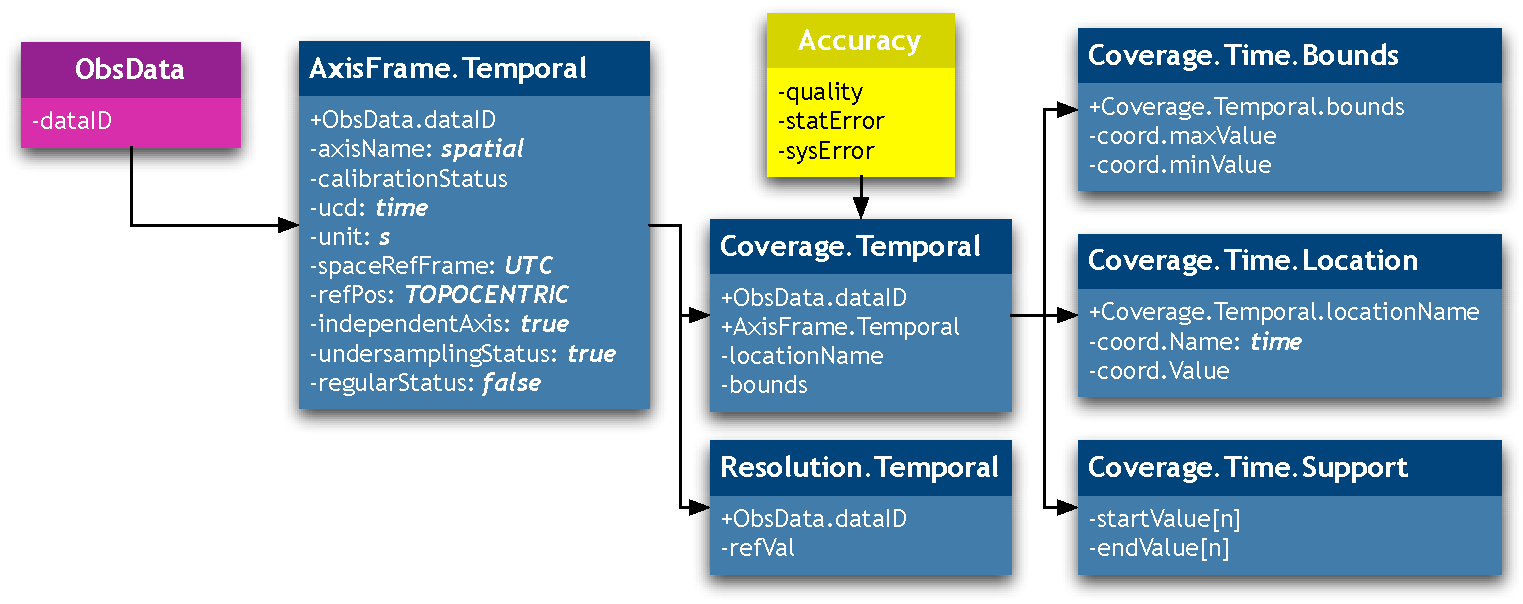
\includegraphics[width=\columnwidth]
				{fig/AxisFrame-Temporal-DM}
				\end{center}
				\caption[Temporal axis metadata]{
					Temporal axis and related coverage metadata.
				}
				\label{figAxisFrameTemporal}
			\end{figure}
			
			\begin{description}
				\item[AxisFrame.Temporal] Describes the 
				properties of the time axis, such as whether the
				axis is calibrated or not ({calibrationStatus}),
				units, reference system ({refPos}), time-scale
				({timescale}), whether the axis is sampled or not
				({undersamplingStatus}), and if sampled, whether
				sampling is regular or not ({samplingStatus}). In
				the case of spectroscopic data, time is not
				sampled.
				
				 We will use the {independentAxis} attribute to
				signal axis dependency as true for continuum
				observations.
				
				 \item[Coverage.Temporal] Collects all the temporal
				characterisation of the observational data.
				
				 \item[Coverage.Temporal.Location]
				Location instances hold the most representative
				value for each axis. For the temporal axis, it holds
				the time of observation, either the starting time
				or the time at the middle of the observation.
				
				 \item[Coverage.Temporal.Bounds] Bounds instances
				hold the maximum and minimum values for the axis.
				In the temporal axis, this is defined as the
				complete observation interval; alternatively, the
				total integration time can be used.
				
				 \item[Coverage.Temporal.Support] Coverage.Support
				instances provide the regions of an axis holding
				observational data. In the temporal axis, this are
				the time intervals actually devoted to flux
				collection\footnote{Actual execution time for each
				individual sub-scan.}.
				
				 \item[Coverage.Temporal.Sensitivity] In cases
				where an instrument had a sensor ramp-up, where
				some time is needed before 100\% sensitivity is
				achieved, this class would describe such a ramp,
				and would allow for convenient scaling of data
				taken during those intervals. If that were never
				the case, Temporal.Sensitivity could just be
				dropped.
				
				 \item[Resolution.Temporal] Holds the temporal
				resolution of the data. Most of the time, telescope
				control system time-stamps are expressed in UTC or
				LST in seconds, so temporal resolution would be of
				the order of a second, but normally the instrument
				could deliver better temporal resolution. We should
				address this after the initial setup.
				
				 We will not develop the SamplingPrecision.Temporal
				class, because we are not sampling the temporal
				axis.
				
				\item[Accuracy.Temporal] This class has to collect
				systematic and statistical errors associated with
				the temporal coordinates of the data. The Quality
				attribute gives additional information about the
				temporal data quality. We could use time re-syncing
				statistics in order to evaluate accuracy.
			\end{description}
			
			
			\begin{table}
			\begin{minipage}{\linewidth}
			\caption[AxisFrame.Temporal metadata]{AxisFrame.Temporal metadata.}
			\begin{smallertabular}{p{3.15 cm}p{1.5cm}p{2.25cm}p{4.35cm}}
						  & \textbf{FITS} & & \\ \textbf{Attribute} &
			              \textbf{Keyword} & \textbf{UCD} &
			              \textbf{Description}\\ \midrule axisName
			              & \texttt{assign} & \texttt{meta.id;
			              meta.main} & Axis name.\\ \addlinespace
			              calibrationStatus & \texttt{assign} &
			              \texttt{time; obs.calib; meta.code} &
			              Calibration status from a controlled
			              vocabulary: \texttt{un\-cal\-i\-brated},
			              \texttt{cal\-i\-brated},
			              \texttt{rel\-a\-tive}\footnote{\texttt{rel\-a\-tive}
			              refers to calibrated data, except for an
			              additive or multiplicative constant.} ,
			              \texttt{nor\-mal\-ized}\footnote{\texttt{normalized}
			              refers to dimensionless quantities, such as
			              those resulting from the division between two
			              commensurable datasets.} \\ \addlinespace ucd &
			              \texttt{assign} & \texttt{time; meta.ucd;
			              meta.main} & Main UCD for the axis.\\ \addlinespace
			              unit & \texttt{assign} & \texttt{time;
			              meta.unit; meta.main} & Main units for the
			              axis.\\ \addlinespace refPos & \texttt{assign} &
			              \texttt{time; meta.ref; meta.id} &
			              Identification of the origin position from a
			              controlled vocabulary.\\ \addlinespace
			              independentAxis & \texttt{assign} &
			              \texttt{time; obs.param; meta.code} & Boolean
			              flag indicating whether the axis is
			              independent of the rest or not.\\ \addlinespace
			              undersamplingStatus & \texttt{assign} &
			              \texttt{time; obs.param; meta.code} & Boolean
			              flag indicating whether the data are sampled
			              in this axis or not.\\ \addlinespace regularStatus &
			              \texttt{assign} & \texttt{time; obs.param;
			              meta.code} & Boolean flag used in case of
			              sampled data, indicating whether sampling is
			              regular or not.\\ \addlinespace numBins &
			              \texttt{assign} & \texttt{time; meta.number}
			              & Number of time samples.\\ \addlinespace
			\end{smallertabular}
			\label{tabAxisFrameTemporalMetadata}
			\end{minipage}
			\end{table}
			
			\begin{table}
			\caption[Coverage.Temporal.Location metadata]
			{Coverage.Temporal.Location metadata.}
			\begin{smallertabular}{p{2.15 cm}p{1.5cm}p{2.25cm}p{5.35cm}}
								& \textbf{FITS} & & \\ \textbf{Attribute} &
			                    \textbf{Keyword} & \textbf{UCD} &
			                    \textbf{Description}\\ \midrule coord.name &
			                    \texttt{assign} & \texttt{time; meta.name} & Name
			                    of the coordinate whose value goes in
			                    coord.value; in this case, \texttt{time} with
			                    respect to refPos. \\ \addlinespace coord.value &
			                    \texttt{assign} & \texttt{time; meta.number} &
			                    Numeric value for the time location; usually, a
			                    MJD or decimal UTC time. \\ \addlinespace
			\end{smallertabular}
			\label{tabCoverageTemporalLocationMetadata}
			\end{table}
			
			\begin{table}
			\begin{minipage}{\linewidth}
			\caption[Coverage.Temporal.Bounds metadata]
			{
					Coverage.Temporal.Bounds metadata\footnote{The UCDs for
			        coord.maxValue and coord.minValue could have been,
			        respectively, \texttt{time.obs.start} and
			        \texttt{time.obs.end}, but we think the proposed UCDs are more
			        consistent with the rest of the axes. Besides, we can defer the
			        election, by using \texttt{time.obs.start} and
			        \texttt{time.obs.end} at the beginning of the UCD, and
			        appending \texttt{meta.number; stat.max} or
			        \texttt{meta.number; stat.min} as additional qualifiers.}.
			}
			\begin{smallertabular}{p{2.15 cm}p{1.5cm}p{2.25cm}p{5.35cm}}
								& \textbf{FITS} & & \\ \textbf{Attribute} &
			                    \textbf{Keyword} & \textbf{UCD} &
			                    \textbf{Description}\\ \midrule coord.name &
			                    \texttt{assign} & \texttt{time; meta.name} & Name
			                    of the coordinate whose maximum and minimum
			                    values go in coord.maxValue and coord.minValue.\\
			                    \addlinespace coord.maxValue & \texttt{assign} &
			                    \texttt{time; meta.number; stat.max} & Minimum
			                    numeric value for the observation time.\\ \addlinespace
			                    coord.minValue & \texttt{assign} & \texttt{time;
			                    meta.number; stat.min} & Maximum numeric value
			                    for the observation time.\\ \addlinespace
			\end{smallertabular}
			\label{tabCoverageTemporalBoundsMetadata}
			\end{minipage}
			\end{table}
			
			\begin{table}
			\begin{minipage}{\linewidth}
			\caption[Coverage.Temporal.Support metadata]
			{
					Coverage.Temporal.Support
			        metadata\footnote{Coverage.Temporal.Support could be
			        alternatively defined by using just one value, the exposure
			        time, with UCD \texttt{time.expo}. The chosen definition, apart
			        from being more consistent across axes, allows for
			        discontinuous temporal support.}.
			}
			\begin{smallertabular}{p{2.15 cm}p{1.5cm}p{2.25cm}p{5.35cm}}
								& \textbf{FITS} & & \\ \textbf{Attribute} &
			                    \textbf{Keyword} & \textbf{UCD} &
			                    \textbf{Description}\\ \midrule code &
			                    \texttt{assign} & \texttt{time; meta.code} & Code
			                    for the time interval where we will be defining
			                    support; an array of [coord.code, startValue,
			                    endValue] tuples can be used to define temporal
			                    support.\\ \addlinespace startValue & \texttt{assign} &
			                    \texttt{time.expo.start} & Time interval start
			                    value.\\ \addlinespace endValue & \texttt{assign} &
			                    \texttt{time.expo.end} & 2DTime interval end
			                    value.\\ \addlinespace
			\end{smallertabular}
			\label{tabCoverageTemporalSupportMetadata}
			\end{minipage}
			\end{table}
			
			\begin{table}
			\caption[Coverage.Temporal.Resolution metadata]
			{Coverage.Temporal.Resolution metadata.}
			\begin{smallertabular}{p{2.15 cm}p{1.5cm}p{2.25cm}p{5.35cm}}
								& \textbf{FITS} & & \\ \textbf{Attribute} &
			                    \textbf{Keyword} & \textbf{UCD} &
			                    \textbf{Description}\\ \midrule
			                    referenceValue & \texttt{assign} & \texttt{time;
			                    meta.number; meta.ref} & Resolution reference
			                    value.\\ \addlinespace
			\end{smallertabular}
			\label{tabCoverageTemporalResolutionMetadata}
			\end{table}
			
			\begin{table}
			\caption[Accuracy.Temporal metadata]{Accuracy.Temporal metadata.}
			\begin{smallertabular}{p{2.15 cm}p{1.5cm}p{2.25cm}p{5.35cm}}
								& \textbf{FITS} & & \\ \textbf{Attribute} &
			                    \textbf{Keyword} & \textbf{UCD} &
			                    \textbf{Description}\\ \midrule quality &
			                    \texttt{assign} & \texttt{time; meta.code.qual} &
			                    Quality code for time coordinates; invalid data
			                    are flagged with a quality code of 1.\\ \addlinespace
			                    sysError & \texttt{assign} & \texttt{time;
			                    stat.error.sys} & Systematic error for time
			                    coordinates.\\ \addlinespace sysErrorHigh &
			                    \texttt{assign} & \texttt{time; stat.error.sys;
			                    stat.max} & Maximum systematic error for time
			                    coordinates.\\ \addlinespace sysErrorLow &
			                    \texttt{assign} & \texttt{time; stat.error.sys;
			                    stat.min} & Minimum systematic error for time
			                    coordinates.\\ \addlinespace statError & \texttt{assign}
			                    & \texttt{time; stat.error} & Statistical error
			                    for time coordinates.\\ \addlinespace statErrorHigh&
			                    \texttt{assign} & \texttt{time; stat.error;
			                    stat.max} & Maximum statistical error for time
			                    coordinates.\\ \addlinespace statErrorLow &
			                    \texttt{assign} & \texttt{time; stat.error;
			                    stat.min} & Minimum statistical error for time
			                    coordinates.\\ \addlinespace
			\end{smallertabular}
			\label{tabAccuracyTemporalMetadata}
			\end{table}
			
		% subsection ssubTemporalAxis (end)
		
		\subsection{AxisFrame.Spectral and Coverage.Spectral} %(fold)
		\label{subSpectralAxis}
			
			In this subsection, we describe the classes that
			configure the description of the spectral axis
			(AxisFrame.Spectral), and the characterisation of the
			coverage in such axis (Coverage.Spectral).
			Figure~\ref{figAxisFrameSpectral} shows the classes and
			their relationships.
			
			\begin{figure}[tbp]
			\begin{center}
			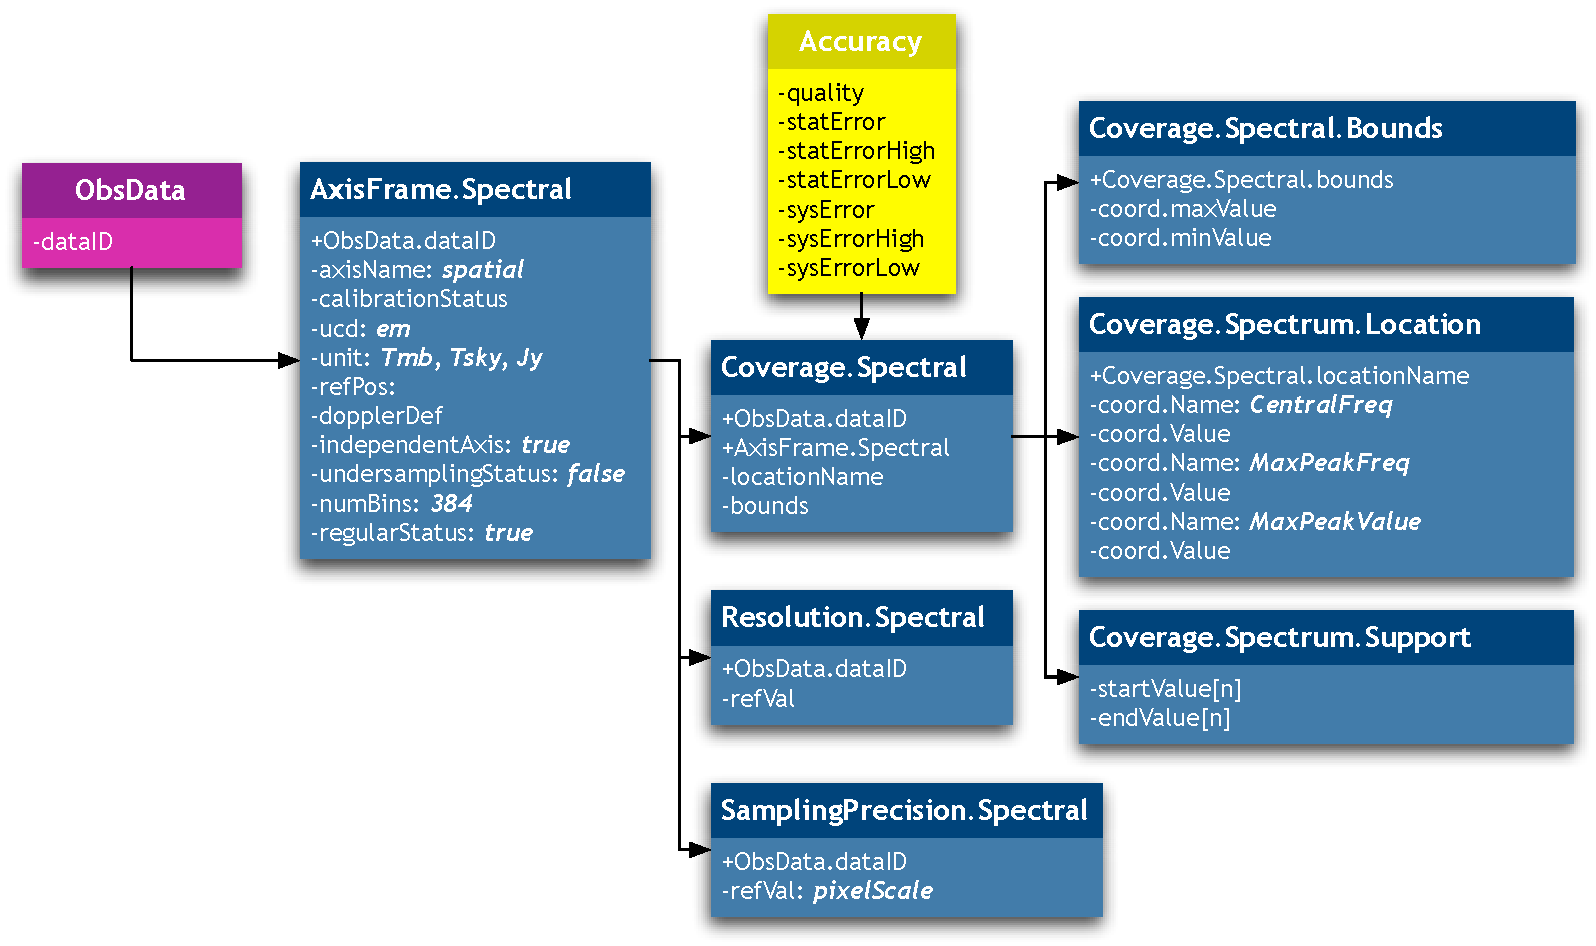
\includegraphics[width=\columnwidth]
			{fig/AxisFrame-Spectral-DM}
			\end{center}
			\caption[Spectral axis metadata]{
				Spectral axis and related coverage metadata.
			}
			\label{figAxisFrameSpectral}
			\end{figure}

			\begin{description}
				\item[AxisFrame.Spectral] Describes the 
				properties of the spectral axis, such as whether the
				axis is calibrated or not (calibrationStatus),
				units, reference system (RefPos), or the
				mathematical definition used for the Doppler effect
				(DopplerDef), for velocity calibrated
				spectra\footnote{For systems in the local standard
				of rest (LSR), emission lines occur at a precise
				frequency. Due do the Doppler effect, systems
				receding from the LSR will show a lower frequency,
				and those approaching will show higher frequencies.
				In the case of complex dynamics, the net effect is
				a broadening of the line, and the Doppler effect
				allows us to calibrate emission at different
				frequencies as emission at different velocities.}.
				It is clear that spectral information is indeed
				sampled, and the number of channels will be coded
				by numBins.
				
				 \item[Coverage.Spectral] Collects the different
				spectral properties of the data.
				
				 \item[Coverage.Spectral.Location]
				Coverage.Location holds the most representative
				value for the axis. In the spectral axis, and being
				a sampled axis, we will use the frequency for the
				central sample of the spectrum.
				
				 \item[Coverage.Spectral.Bounds] Holds the spectral
				limits of the data, that is, the starting and
				ending frequency for the spectrum.
				
				 \item[Coverage.Spectral.Support] Holds the
				spectral support for the data. We could choose to
				register just the actual bandwidth, or better, to
				set an array of different intervals where the
				instrument is sensitive. Better yet, we could
				register a sensitivity profile for each frequency.
				We will initially choose the array of intervals as
				the way to express the spectral support.
				
				 \item[Coverage.Spectral.Sensitivity] Holds the
				sensitivity profile for the instrument in
				frequency; in other words, this would be equal to
				the detailed frequency response of the whole
				antenna-receiver-backend set.
				
				 \item[Resolution.Spectral] Holds the spectral
				resolution information for the data. For filter
				banks, it is the filter bandwidth for each filter,
				or an average filter bandwidth. In the case of
				spectra obtained from the Fourier transform of the
				autocorrelation function, it is equal to the
				bandwidth divided by the number of channels.
				
				 \item[SamplingPrecision.Spectral] In the case of
				the Robledo antenna, this value should be equal to
				the value stored at Resolution.Spectral. For other
				instruments, SamplingPrecision.Spectral defines the
				frequency steps from one frequency bin to the next.
				
				 \item[Accuracy.Spectral] Errors associated with
				the spectrum. In the same way as the support could
				change along the spectrum, because of different
				sensitivities, we might need to characterise the
				accuracy along the spectrum. At least in the case
				of Robledo, the SNR is global, and considered equal
				for all frequencies. If not, a first approximation
				can be using an average SNR, and maximum and
				minimum SNR.
			\end{description}
			
			\begin{table}
			\begin{minipage}{\linewidth}
			\caption[AxisFrame.Spectral metadata]{AxisFrame.Spectral metadata.}
			\begin{smallertabular}{p{3.05 cm}p{1.5cm}p{2.85cm}p{3.85cm}}
							& \textbf{FITS} & & \\ \textbf{Attribute} &
			                \textbf{Keyword} & \textbf{UCD} &
			                \textbf{Description}\\ \midrule axisName &
			                \texttt{assign} & \texttt{meta.id; meta.main} & Axis
			                name (\texttt{frequency} or \texttt{velocity}).\\
			                \addlinespace calibrationStatus & \texttt{assign} &
			                \texttt{em.radio; obs.calib; meta.code} & Calibration
			                status from a controlled vocabulary:
			                \texttt{un\-cal\-i\-brated}, \texttt{cal\-i\-brated},
			                \texttt{rel\-a\-tive}\footnote{\texttt{rel\-a\-tive}
			                refers to calibrated data, except for an additive or
			                multiplicative constant} ,
			                \texttt{nor\-mal\-ized}\footnote{\texttt{normalized}
			                refers to dimensionless quantities, such as those
			                resulting from the division between two commensurable
			                datasets.}.\\ \addlinespace ucd & \texttt{assign} &
			                \texttt{em.radio; meta.ucd; meta.main} & Main UCD for
			                the axis.\\ \addlinespace unit & \texttt{TUNITn} &
			                \texttt{em.radio; meta.unit; meta.main} & Main units
			                for the axis.\\ \addlinespace refPos & \texttt{assign} &
			                \texttt{em.radio; meta.ref; meta.id} & Identification
			                of the origin position from a controlled
			                vocabulary.\\ \addlinespace dopplerDef & \texttt{VELDEF} &
			                \texttt{spect.dopplerParam; meta.code} & Code
			                defining the type of Doppler shift definition used
			                for frequency and/or velocity calibration; from a
			                controlled vocabulary: \texttt{op\-ti\-cal},
			                \texttt{ra\-di\-o}, \texttt{rel\-a\-tiv\-is\-tic}.\\
			                \addlinespace independentAxis & \texttt{assign} &
			                \texttt{em.radio; obs.param; meta.code} & Boolean
			                flag indicating whether the axis is independent of
			                the rest or not.\\ \addlinespace undersamplingStatus &
			                \texttt{assign} & \texttt{em.radio; obs.param;
			                meta.code} & Boolean flag indicating whether the data
			                are sampled in this axis or not.\\ \addlinespace
			                regularStatus & \texttt{assign} & \texttt{em.radio;
			                obs.param; meta.code} & Boolean flag used in case of
			                sampled data, indicating whether sampling is regular
			                or not.\\ \addlinespace numBins & \texttt{assign} &
			                \texttt{em.radio; meta.number} & Number of spectral
			                samples.\\ \addlinespace
			\end{smallertabular}
			\label{tabAxisFrameSpectralMetadata}
			\end{minipage}
			\end{table}
			
			\begin{table}
			\caption[Coverage.Spectral.Location metadata]
			{Coverage.Spectral.Location metadata.}
			\begin{smallertabular}{p{2.15 cm}p{1.5cm}p{2.25cm}p{5.35cm}}
						& \textbf{FITS} & & \\ \textbf{Attribute} &
			            \textbf{Keyword} & \textbf{UCD} & \textbf{Description}\\
			            \midrule coord.name & \texttt{assign} &
			            \texttt{em.radio; meta.name} & Name of the coordinate
			            whose value goes in coord.value; in this case,
			            \texttt{frequency} with respect to refPos.\\ \addlinespace
			            coord.value & \texttt{OBSFREQ} & \texttt{em.radio;
			            em.freq; stat.mean} & Numeric value for the central
			            frequency location.\\ \addlinespace
			\end{smallertabular}
			\label{tabCoverageSpectralLocationMetadata}
			\end{table}
			
			\begin{table}
			\caption[Coverage.Spectral.Bounds metadata]
			{Coverage.Spectral.Bounds metadata.}
			\begin{smallertabular}{p{2.15 cm}p{1.5cm}p{2.25cm}p{5.35cm}}
						& \textbf{FITS} & & \\ \textbf{Attribute} &
			            \textbf{Keyword} & \textbf{UCD} & \textbf{Description}\\
			            \midrule coord.name & \texttt{assign} &
			            \texttt{em.radio; meta.name} & Name of the coordinate
			            whose maximum and minimum values go in coord.maxValue and
			            coord.minValue.\\ \addlinespace coord.maxValue & \texttt{assign}
			            & \texttt{em.freq; meta.number; stat.max} & Minimum
			            frequency value.\\ \addlinespace coord.minValue &
			            \texttt{assign} & \texttt{em.freq; meta.number; stat.min}
			            & Maximum frequency value.\\ \addlinespace
			\end{smallertabular}
			\label{tabCoverageSpectralBoundsMetadata}
			\end{table}
			
			\begin{table}
			\caption[Coverage.Spectral.Support metadata]
			{Coverage.Spectral.Support metadata.}
			\begin{smallertabular}{p{2.15 cm}p{1.5cm}p{2.25cm}p{5.35cm}}
						& \textbf{FITS} & & \\ \textbf{Attribute} &
			            \textbf{Keyword} & \textbf{UCD} & \textbf{Description}\\
			            \midrule code & \texttt{assign} & \texttt{em.radio;
			            meta.record} & Code for the interval where we will be
			            defining support; an array of [coord.code, startValue,
			            endValue] tuples can be used to define spectral support.\\
			            \addlinespace startValue & \texttt{assign} & \texttt{em.freq;
			            stat.min} & Frequency interval start value.\\ \addlinespace
			            endValue & \texttt{assign} & \texttt{em.freq; stat.max} &
			            Frequency interval end value.\\ \addlinespace
			\end{smallertabular}
			\label{tabCoverageSpectralSupportMetadata}
			\end{table}
			
			\begin{table}
			\caption[Coverage.Spectral.Sensitivity metadata]
			{Coverage.Spectral.Sensitivity metadata.}
			\begin{smallertabular}{p{2.15 cm}p{1.5cm}p{2.25cm}p{5.35cm}}
						& \textbf{FITS} & & \\ \textbf{Attribute} &
			            \textbf{Keyword} & \textbf{UCD} & \textbf{Description}\\
			            \midrule numChannels & \texttt{assign} &
			            \texttt{em.radio; meta.number} & Number of channels of
			            the frequency response of the filter that describes
			            spectral sensitivity.\\ \addlinespace channel[n] &
			            \texttt{assign} & \texttt{em.freq} & Frequency for the
			            n\thsup{} channel of the filter that describes spectral
			            sensitivity.\\ \addlinespace response[n] & \texttt{assign} &
			            \texttt{arith.factor} & Filter response for the n\thsup{}
			            channel.\\ \addlinespace
			\end{smallertabular}
			\label{tabCoverageSpectralSensitivityMetadata}
			\end{table}
			
			\begin{table}
			\begin{minipage}{\linewidth}
			\caption[Coverage.Spectral.Resolution metadata]
			{Coverage.Spectral.Resolution metadata\footnote{When the Sensitivity
			class is provided, Resolution.numChannels has to be equal to
			Sensitivity.numChannels, and each channel can support different
			resolutions. When the Sensitivity class is not provided,
			Resolution.numChannels has to be set to \texttt{1}, and
			Resolution.referenceValue represents the average channel
			resolution.}.}
			\begin{smallertabular}{p{2.15 cm}p{1.5cm}p{2.45cm}p{5.15cm}}
						& \textbf{FITS} & & \\ \textbf{Attribute} &
			            \textbf{Keyword} & \textbf{UCD} & \textbf{Description}\\
			            \midrule numChannels & \texttt{assign} &
			            \texttt{em.radio; meta.number} & Number of channels for
			            which resolution is provided.\\ \addlinespace referenceValue[n]
			            & \texttt{FREQRES} & \texttt{em.freq; spect.resolution} &
			            Resolution reference value for the n\thsup{} channel.\\ \addlinespace
			\end{smallertabular}
			\label{tabCoverageSpectralResolutionMetadata}
			\end{minipage}
			\end{table}
			
			\begin{table}
			\begin{minipage}{\linewidth}
			\caption[SamplingPrecision.Spectral metadata]
			{SamplingPrecision.Spectral metadata\footnote{When
			SamplingPrecision.numChannels is set to \texttt{0}, the number of
			spectral channels is given by AxisFrame.Spectral.numBins, and
			SamplingPrecision provides the sampling step in a single
			referenceValue. Otherwise, SamplingPrecision.Spectral.numBins must be
			equal to AxisFrame.Spectral.numBins, and when the Sensitivity class
			is provided, SamplingPrecision.Spectral.numBins must be equal to
			Spectral.Sensitivity.numChannels, and
			Spectral.SamplingPrecision.referenceValue[n] equal to
			Spectral.Sensitivity.channel[n].}.}
			\begin{smallertabular}{p{2.15 cm}p{1.5cm}p{2.45cm}p{5.15cm}}
						& \textbf{FITS} & & \\ \textbf{Attribute} &
			            \textbf{Keyword} & \textbf{UCD} & \textbf{Description}\\
			            \midrule numChannels & \texttt{assign} &
			            \texttt{em.radio; meta.number} & Number of frequencies
			            that we are sampling.\\ \addlinespace referenceValue[n] &
			            \texttt{FREQRES} & \texttt{em.freq; spect.resolution} &
			            Resolution reference value for the n\thsup{} channel.\\ \addlinespace
			\end{smallertabular}
			\label{tabSamplingPrecisionSpectralMetadata}
			\end{minipage}
			\end{table}
			
			\begin{table}
			\caption[Accuracy.Spectral metadata]{Accuracy.Spectral metadata.}
			\begin{smallertabular}{p{2.15 cm}p{1.5cm}p{2.25cm}p{5.35cm}}
						& \textbf{FITS} & & \\ \textbf{Attribute} &
			            \textbf{Keyword} & \textbf{UCD} & \textbf{Description}\\
			            \midrule quality & \texttt{assign} &
			            \texttt{em.freq; meta.code.qual} &Quality code for
			            frequency coordinates; invalid data are flagged with a
			            quality code of 1.\\ \addlinespace sysError & \texttt{assign} &
			            \texttt{em.freq; stat.error.sys} &Systematic error for
			            frequency coordinates.\\ \addlinespace sysErrorHigh &
			            \texttt{assign} & \texttt{em.freq; stat.error.sys;
			            stat.max} & Maximum systematic error for frequency
			            coordinates.\\ \addlinespace sysErrorLow & \texttt{assign} &
			            \texttt{em.freq; stat.error.sys; stat.min} & Minimum
			            systematic error for frequency coordinates.\\ \addlinespace
			            statError & \texttt{assign} & \texttt{em.freq;
			            stat.error} &Statistical error for frequency
			            coordinates.\\ \addlinespace statErrorHigh& \texttt{assign} &
			            \texttt{em.freq; stat.error; stat.max} & Maximum
			            statistical error for frequency coordinates.\\ \addlinespace
			            statErrorLow & \texttt{assign} & \texttt{em.freq;
			            stat.error; stat.min} & Minimum statistical error for
			            frequency coordinates.\\ \addlinespace
			\end{smallertabular}
			\label{tabAccuracySpectralMetadata}
			\end{table}
			
		% subsection subSpectralAxis (end)

		\subsection{AxisFrame.Observable and Coverage.Observable} %(fold)
		\label{ssubObservableAxis}
			
			The Observable axis is, finally, the one directly
			related to the stored data, instead of data headers. In
			this subsection, we describe the classes that configure
			the description of the observable axis
			(AxisFrame.Observable), and the characterisation of the
			coverage in such axis (Coverage.Observable).
			Figure~\ref{figAxisFrameObservable} shows the classes
			and their relationships.
			
			\begin{figure}[tbp]
			\begin{center}
				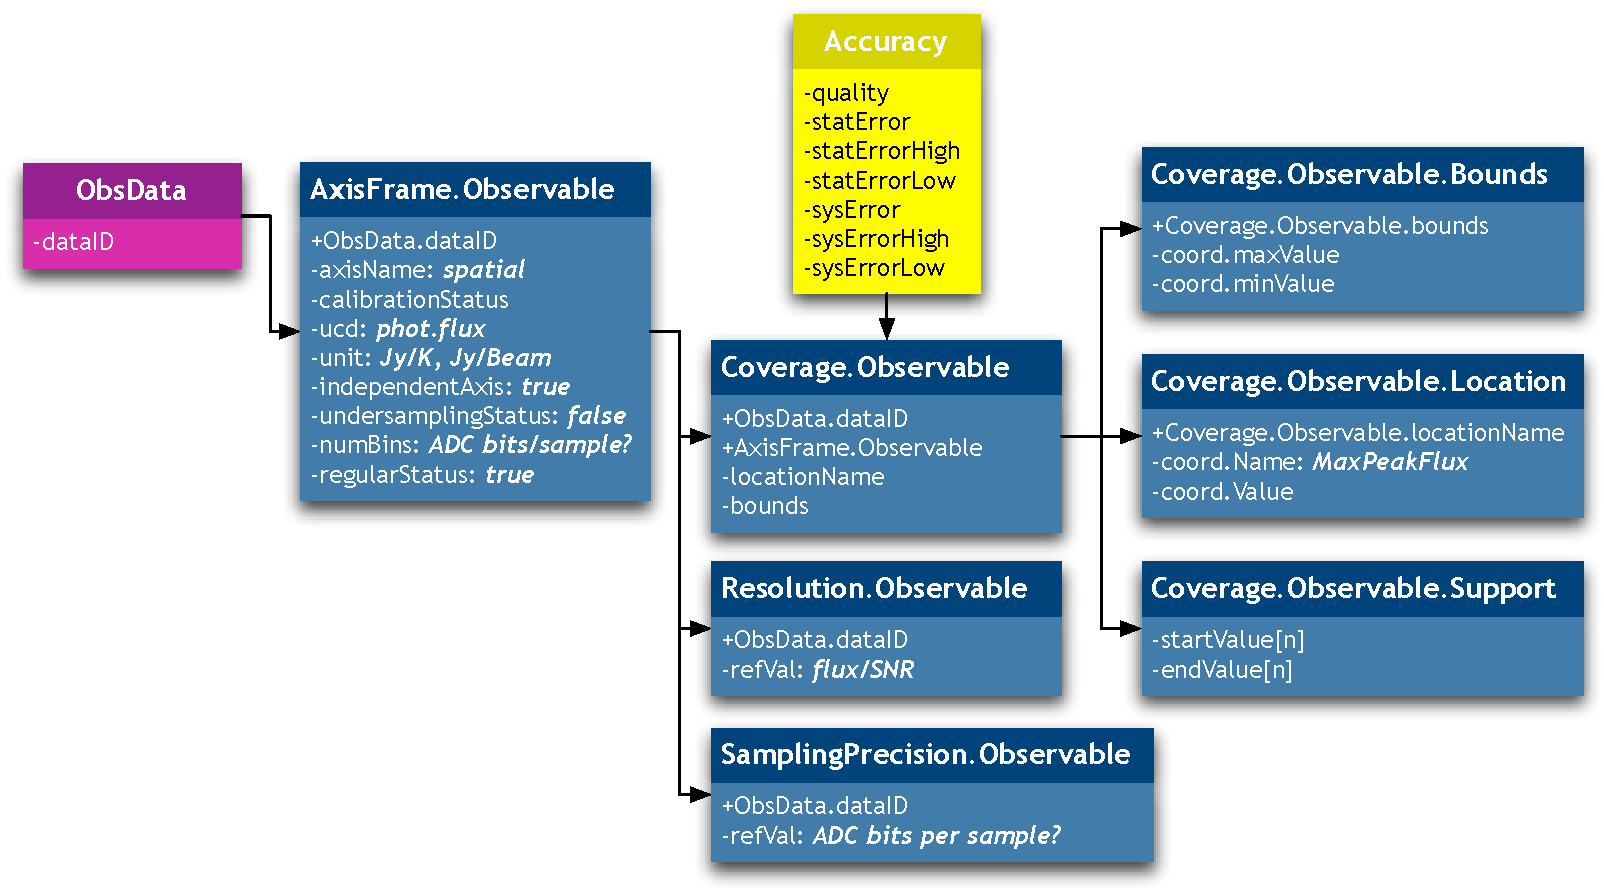
\includegraphics[width=\columnwidth]
				{fig/AxisFrame-Observable-DM}
			\end{center}
			\caption[Observable axis metadata]
			{Observable axis and related coverage metadata.}
			\label{figAxisFrameObservable}
			\end{figure}

			\begin{description}
				\item[AxisFrame.Observable] Describes the 
				properties of the observable axis (whether the
				observable is flux,
				polarisation state, or any other), such as whether
				the data is calibrated or not (calibrationStatus),
				applicable units, et cetera. Flux information is
				sampled at the digital conversion stage, and the
				number of available different flux levels is
				codified in numBins. By specifying units in this
				class, we define whether the observable data are
				provided in flux units, or in brightness or antenna
				temperature. Additional information, such as the
				polarisation, can be accommodated in the same axis
				in the same way we extended the Spatial axis for 2D
				or 3D coordinates, or by means of (an) additional
				observable (axis) axes.
				
				 \item[Coverage.Observable] Collects all
				information that directly characterises observable
				data.
				
				 \item[Coverage.Observable.Location]
				Coverage.Location instances hold the most
				representative value for that axis. In this case,
				the average spectrum flux is not significant,
				specially if we have a strong line detection.
				Hence, for this axis we will take the maximum flux
				as Observable.Location.
				
				 \item[Coverage.Observable.Bounds] Coverage.Bounds
				instances record the maximum and minimum values for
				the axis. In the Observable axis, it records
				minimum and maximum flux for the spectrum.
				
				 \item[Coverage.Observable.Support] This instance
				should give us the intervals of flux observed in
				the spectrum, and we could choose between making it
				equal to Coverage.Observable.Bounds, or defining an
				interval that holds a given dispersion from the
				Coverage.Observable.Location value. We will
				initially consider Coverage.Observable.Support as
				equal to Coverage.Observable.Bounds.
				
				 \item[Coverage.Observable.Sensitivity] This would
				store the change rate in the observable axis for a
				given observed flux.
				
				 \item[Resolution.Observable] We keep the flux
				resolution for the data, defined as mean flux
				divided by the SNR, or mean noise.
				
				 \item[SamplingPrecision.Observable] Instances of
				this class indicate the sampling precision. For the
				observable (flux) axis, this should be equal to the
				Analog to Digital Converter (ADC) resolution, or
				worse if more processing is involved, and should be
				tabulated by instrument setup. We might also
				consider this axis as non-sampled, as
				Resolution.Observable is usually well above ADC
				resolution, and drop this class.
				
				 \item[Accuracy.Observable] Collected flux
				associated errors. Errors on the observable axis
				can be dependent on received flux, and so we should
				give an average value, and either variance or
				maximum and minimum accuracy on the observable
				axis.
				
				 If the observable variable were a different one,
				the main difference would correspond to the change
				of UCDs. In the particular case of polarisation,
				\texttt{phot.flux} would be replaced by
				\texttt{phys.polarization}. Other changes would
				include an additional characterisation of the
				parameters been actually returned by the
				instrument, and their relationship with Stokes
				parameters.
			\end{description}
			
			\begin{table}
			\begin{minipage}{\linewidth}
			\caption[AxisFrame.Observable metadata]
			{AxisFrame.Observable metadata (when the observed variable is flux).}
			\begin{smallertabular}{p{3.15 cm}p{1.5cm}p{2.25cm}p{4.35cm}}
						& \textbf{FITS} & & \\ \textbf{Attribute} &
			            \textbf{Keyword} & \textbf{UCD} & \textbf{Description}\\
			            \midrule axisName & \texttt{assign} &
			            \texttt{meta.id; meta.main} & Axis name.\\ \addlinespace
			            calibrationStatus & \texttt{assign} & \texttt{em.radio;
			            obs.calib; meta.code} & Calibration status from a
			            controlled vocabulary: \texttt{un\-cal\-i\-brated},
			            \texttt{cal\-i\-brated},
			            \texttt{rel\-a\-tive}\footnote{\texttt{rel\-a\-tive}
			            refers to calibrated data, except for an additive or
			            multiplicative constant} ,
			            \texttt{nor\-mal\-ized}\footnote{\texttt{nor\-ma\-lized}
			            refers to dimensionless quantities, such as those
			            resulting from the division between two commensurable
			            datasets.}.\\ \addlinespace ucd & \texttt{assign} &
			            \texttt{phot.flux; meta.ucd; meta.main} & Main UCD for
			            the axis.\\ \addlinespace unit & \texttt{TUNITn} &
			            \texttt{phot.flux; meta.unit; meta.main} & Main units for
			            the axis.\\ \addlinespace refPos & \texttt{assign} &
			            \texttt{phot.flux; meta.ref; meta.id} & Identification of
			            the origin position from a controlled vocabulary.\\
			            \addlinespace independentAxis & \texttt{assign} &
			            \texttt{phot.flux; obs.param; meta.code} & Boolean flag
			            indicating whether the axis is independent of the rest or
			            not.\\ \addlinespace undersamplingStatus & \texttt{assign} &
			            \texttt{phot.flux; obs.param; meta.code} & Boolean flag
			            indicating whether the data are sampled in this axis or
			            not.\\ \addlinespace regularStatus & \texttt{assign} &
			            \texttt{phot.flux; obs.param; meta.code} & Boolean flag
			            used in case of sampled data, indicating whether sampling
			            is regular or not.\\ \addlinespace numBins & \texttt{assign} &
			            \texttt{phot.flux; meta.number} & Number of spectral
			            samples (if the axis is sampled)\\ \addlinespace
			\end{smallertabular}
			\label{tabAxisFrameObservableMetadata}
			\end{minipage}
			\end{table}
			
			\begin{table}
			\caption[Coverage.Observable.Location metadata]
			{Coverage.Observable.Location metadata (when the observed variable is
			flux).}
			\begin{smallertabular}{p{2.15 cm}p{1.5cm}p{2.25cm}p{5.35cm}}
						& \textbf{FITS} & & \\ \textbf{Attribute} &
			            \textbf{Keyword} & \textbf{UCD} & \textbf{Description}\\
			            \midrule coord.name & \texttt{assign} &
			            \texttt{phot.flux; meta.name} & Name of the coordinate
			            whose value goes in coord.value; in this case,
			            \texttt{flux} with respect to refPos.\\ \addlinespace
			            coord.value & \texttt{assign} & \texttt{phot.flux;
			            stat.max} & Numeric value for the maximum flux (flux
			            location).\\ \addlinespace
			\end{smallertabular}
			\label{tabCoverageObservableLocationMetadata}
			\end{table}
			
			\begin{table}
			\caption[Coverage.Observable.Bounds metadata]
			{Coverage.Observable.Bounds metadata.}
			\begin{smallertabular}{p{2.15 cm}p{1.5cm}p{2.25cm}p{5.35cm}}
						& \textbf{FITS} & & \\ \textbf{Attribute} &
			            \textbf{Keyword} & \textbf{UCD} & \textbf{Description}\\
			            \midrule coord.name & \texttt{assign} &
			            \texttt{phot.flux; meta.name} & Name of the coordinate
			            whose maximum and minimum values go in coord.maxValue and
			            coord.minValue.\\ \addlinespace coord.maxValue & \texttt{assign}
			            & \texttt{phot.flux; stat.max} & Minimum flux value.\\
			            \addlinespace coord.minValue & \texttt{assign} &
			            \texttt{phot.flux; stat.min} & Maximum flux value.\\
			            \addlinespace
			\end{smallertabular}
			\label{tabCoverageObservableBoundsMetadata}
			\end{table}
			
			\begin{table}
			\caption[Coverage.Observable.Support metadata]
			{Coverage.Observable.Support metadata
			(when the observed variable is flux).}
			\begin{smallertabular}{p{2.15 cm}p{1.5cm}p{2.25cm}p{5.35cm}}
						& \textbf{FITS} & & \\ \textbf{Attribute} &
			            \textbf{Keyword} & \textbf{UCD} & \textbf{Description}\\
			            \midrule code & \texttt{assign} & \texttt{em.radio;
			            meta.record} & Code for the interval where we will be
			            defining support; an array of [coord.code, startValue,
			            endValue] tuples can be used to define spectral support.\\
			            \addlinespace startValue & \texttt{assign} & \texttt{em.freq;
			            stat.min} & Frequency interval start value.\\ \addlinespace
			            endValue & \texttt{assign} & \texttt{em.freq; stat.max} &
			            Frequency interval end value.\\ \addlinespace
			\end{smallertabular}
			\label{tabCoverageObservableSupportMetadata}
			\end{table}
			
			%\begin{table}
			%\caption[Coverage.Observable.Sensitivity metadata]
			%{Coverage.Observable.Sensitivity metadata.}
			%\begin{smallertabular}{p{2.15 cm}p{1.5cm}p{2.25cm}p{5.35cm}}
			%			& \textbf{FITS} & & \\ \textbf{Attribute} &
			%            \textbf{Keyword} & \textbf{UCD} & \textbf{Description}\\
			%            \hline \hline
			%\end{smallertabular}
			%\label{tabCoverageObservableSensitivityMetadata}
			%\end{table}
			
			\begin{table}
			\caption[Coverage.Observable.Resolution metadata]
			{Coverage.Observable.Resolution metadata.}
			\begin{smallertabular}{p{2.15 cm}p{1.5cm}p{2.25cm}p{5.35cm}}
						& \textbf{FITS} & & \\ \textbf{Attribute} &
			            \textbf{Keyword} & \textbf{UCD} & \textbf{Description}\\
			            \midrule referenceValue & \texttt{assign} &
			            \texttt{phot.flux; stat.snr; arith.ratio} & Flux
			            resolution (Flux/SNR), as $$\mathrm{\frac{Flux}{SNR} =
			            flux \times \frac{fluxNoise}{fluxSignal}}.$$ Equivalent
			            to average noise.\\ \addlinespace
			\end{smallertabular}
			\label{tabCoverageObservableResolutionMetadata}
			\end{table}
			
			\begin{table}
			\begin{minipage}{\linewidth}
			\caption[SamplingPrecision.Observable metadata]
			{SamplingPrecision.Observable metadata\footnote{Somewhat redundant,
			given the presence of AxisFrame.Observable.numBins. However, we
			include it for completeness.}.}
			\begin{smallertabular}{p{2.15 cm}p{1.5cm}p{2.25cm}p{5.35cm}}
						& \textbf{FITS} & & \\ \textbf{Attribute} &
			            \textbf{Keyword} & \textbf{UCD} & \textbf{Description}\\
			            \midrule referenceValue & \texttt{assign} &
			            \texttt{phot.flux; instr.precision} & Flux sampling
			            precision; maybe expressed as the number of bits per
			            sample.\\ \addlinespace
			\end{smallertabular}
			\label{tabSamplingPrecisionObservableMetadata}
			\end{minipage}
			\end{table}
			
			\begin{table}
			\caption[Accuracy.Observable metadata]{Accuracy.Observable metadata.}
			\begin{smallertabular}{p{2.15 cm}p{1.5cm}p{2.25cm}p{5.35cm}}
						& \textbf{FITS} & & \\ \textbf{Attribute} &
			            \textbf{Keyword} & \textbf{UCD} & \textbf{Description}\\
			            \midrule quality & \texttt{assign} &
			            \texttt{phot.flux; meta.code.qual} &Quality code for the
			            observed flux; invalid data are flagged with a quality
			            code of 1.\\ \addlinespace sysError & \texttt{assign} &
			            \texttt{phot.flux; stat.error.sys} &Systematic error for
			            the observed flux.\\ \addlinespace sysErrorHigh &
			            \texttt{assign} & \texttt{phot.flux; stat.error.sys;
			            stat.max} & Maximum systematic error for the observed
			            flux.\\ \addlinespace sysErrorLow & \texttt{assign} &
			            \texttt{phot.flux; stat.error.sys; stat.min} & Minimum
			            systematic error for the observed flux.\\ \addlinespace
			            statError & \texttt{assign} & \texttt{phot.flux;
			            stat.error} &Statistical error for the observed flux.\\
			            \addlinespace statErrorHigh& \texttt{assign} &
			            \texttt{phot.flux; stat.error; stat.max} & Maximum
			            statistical error for the observed flux.\\ \addlinespace
			            statErrorLow & \texttt{assign} & \texttt{phot.flux;
			            stat.error; stat.min} & Minimum statistical error for the
			            observed flux.\\ \addlinespace
			\end{smallertabular}
			\label{tabAccuracyObservableMetadata}
			\end{table}
			
		% subsection ssubObservableAxis (end)

	% section subObsDataCharacterisation (end)


	\section{Target} % (fold)
	\label{subTargetDesc}
		\attributedquote{
			\dictionarydef
				{target}
				{noun}
				{
					\begin{itemize}
						\item a person, object, or place selected as
						the aim of an attack.
						
						\item a mark or point at which someone fires
						or aims, especially a round or rectangular 
						board marked with concentric circles used in
						archery or shooting.
					\end{itemize}
				}
				\dictionarydef
					{on target}
					{phrase}
					{
						\begin{itemize}
							\item accurately hitting the thing
							aimed at.
						\end{itemize}
					}
		}
		{The New  Oxford American Dictionary, \emph{2nd Edition}}
		
		
		\noindent
		It is necessary to have a systematic storage of the targets
		being studied, because we have to allow queries by
		previously studied targets, as it is very likely that
		this query will be the most used one.
		
		\begin{figure}[tbp]
			\begin{center}
				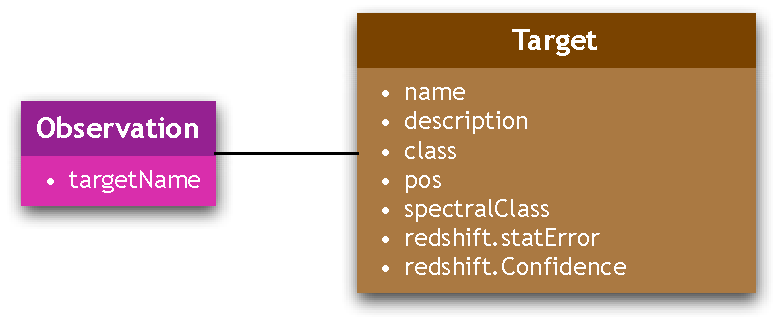
\includegraphics[width=0.5\columnwidth]
				{fig/Target-DM}
			\end{center}
			\caption[Target data model]{Target data model.}
			\label{figTargetDataModel}
		\end{figure}

		The ObsDM distinguishes between
		several types of targets:

		\begin{description}
			\item[Astronomical object] It is a target for which
			some properties are known before the observation.
			
			 \item[Source] An entity created after analysing an
			observation; represents the actual detection by an
			instrument.
			
			 \item[Field] A region of the sky, not a single point
			or collection of points.
			
			 \item[Pointing target] A particular location for an
			observation. It can be part of an Astronomical object,
			a Field, or other entities, such as a Calibrator.
		\end{description}

		IVOA has not developed the Target class as a whole, but the
		authors of the SDM~\cite{McDowell:2006fk} have developed a
		set of possible metadata. We will initially adopt that set
		for the RADAMS, and we can see the associated metadata in
		Figure~\ref{figTargetDataModel}.
		
		Another data model dealing with Targets is the Resource
		Data Model~\cite{2004ASPC..314..273H}, which considers
		additional targets for observations, such as radio flux
		calibrators, pointing calibrators, et cetera.
		
		We have to take into account that most of the time the
		archive will store ObsData associated to Pointing targets,
		but said Pointing targets can also be related to
		Astronomical Objects.
		\invisiblenote{E.g., in the scientific case we
		mentioned in section~\ref{subScientificCase}, the dish is
		pointed to a Pointing target in order to find a maser, but
		that Pointing target will be most likely included within an
		Astronomical object, such as a planetary nebula.}
		For instance, an astronomer might have a program in which
		s/he is looking for water masers as tracers of shocked
		regions, and specifies several Pointing targets. Those
		Pointing targets, however, will be most likely found within
		an Astronomical object, such as a planetary nebula. The
		association of the Astronomical object and the Pointing
		target will be made by means of the Target class.
		
	% section subTargetDesc (end)
	
	
	\section{Conclusions} % (fold)
	\label{sec:radams_cha_conclusions}
		
		In this chapter we have shown that the already specified
		IVOA data models for Characterisation, together with the
		Target data model, do not need to be altered in order to
		be used for radio astronomical archives.
		
		However, the UCDs for data in the ObsDM, CharDM, or in the
		Target class had never been specified before, and this
		contributes to the better interoperation of archives, as
		data with the same UCDs can be interesting for use in
		automatic data mining and data discovery.
		
		In the next chapters we will analyse the parts of the RADAMS
		which need to be created in order to support radio
		astronomical archives.
		
	% section radams_cha_conclusions (end)
	
% chapter radamscharobs (end)